% !TEX root =  MAIN.tex

\newpage
\subsection{Test Suite Augmentation for Space Software Pipeline}
\label{sec:semus}

Symbolic Execution-based Mutant analysis for Space software (FAQAS-SEMuS), is an extension of SEMu that implements test generation for space software. 

\begin{figure}[tb]
\begin{center}
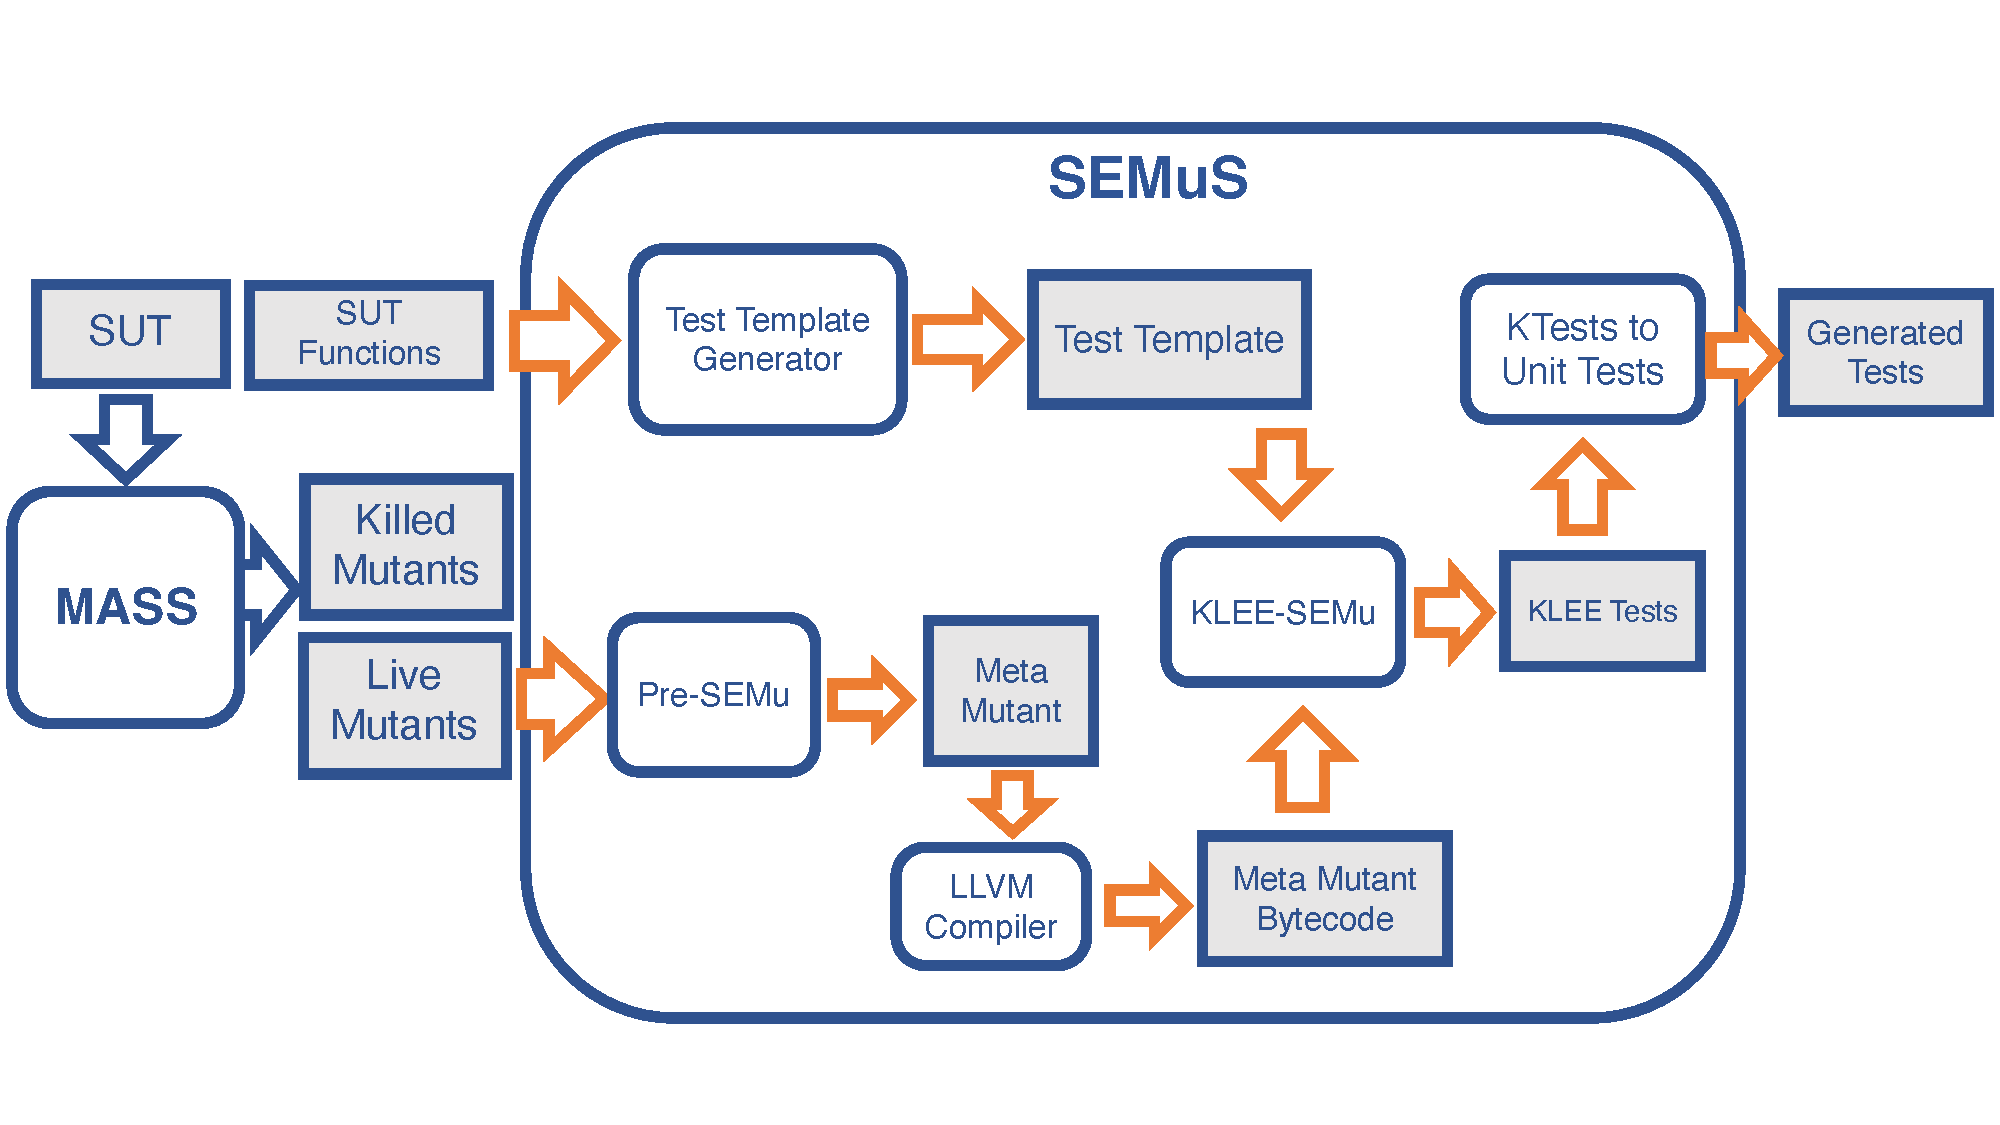
\includegraphics[width=0.8\textwidth]{images/semus-architecture}
\caption{FAQAS-SEMuS Architecture}
\label{fig:semus_architecture}
\end{center}
\end{figure}

Figure~\ref{fig:semus_architecture} shows the architecture of SEMuS and how the tool interacts with MASS.

%SEMuS receives the following inputs: (a) the list of live mutants (produced by MASS), (b) the SUT, and (c) the SUT functions. 

As shown in Figure~\ref{fig:semus_architecture} SEMus is composed by five components, the \emph{Test Template Generator}, the \emph{Pre-SEMu}, the \emph{KLEE-SEMu}, the \emph{KTest to Unit Test}, and the \emph{LLVM}.

% !TEX root =  ../MAIN.tex

\begin{lstlisting}[style=CStyle, caption=SEMuS test template., label=test_template]
int main(int argc, char** argv) {
    // Declare variable to hold function returned value
    _Bool result_faqas_semu; 
    // Declare arguments and make input ones symbolic
    unsigned long pVal;
    int pErrCode;
    klee_make_symbolic(&pVal, sizeof(pVal), "pVal"); // Call function under test
    result_faqas_semu = T_INT_IsConstraintValid(&pVal, &pErrCode); // Make some output
    printf("FAQAS-SEMU-TEST_OUTPUT: %d\n", pErrCode);
    printf("FAQAS-SEMU-TEST_OUTPUT: %d\n", result_faqas_semu);
    return (int)result_faqas_semu;
}

\end{lstlisting}


\begin{lstlisting}[language={}, caption=Klee-test output, label=ktest]
ktest file : 'test000001.ktest'
args       : ['/MakeSym-TestGen-Input/direct/T_INT_IsConstraintValid/test.MetaMu.bc']
num objects: 2
object    0: name: b'model_version'
object    0: size: 4
object    0: data: b'\x01\x00\x00\x00'
object    1: name: b'pVal'
object    1: size: 8
object    1: data: b'\x00\x00\x00\x00\x00\x00\x00\x00'
\end{lstlisting}

The \emph{Test Template Generator} (TTG) component automates the generation of templates for the symbolic execution search. The component receives as inputs the SUT source code and the list of SUT functions. 
Listing~\ref{test_template} shows an example of a test template generated by the TTG. The TTG generates a template for every SUT function; as shown in Listing~\ref{test_template} the component parses the function arguments and declares them symbolic through use of the KLEE function \texttt{klee\_make\_symbolic}. Then, it adds a call to the function under analysis with symbolic values, and it saves the output into the variable \texttt{result\_faqas\_semu}. Finally, the TTG adds a return call with the \texttt{result\_faqas\_semu} variable value.

The \emph{Pre-SEMu} component implements \INDEX{mutant schemata}; specifically, the component includes and compiles all the live mutants (i.e., MASS output) into a single bytecode file named the \emph{Meta Mutant}. At runtime, the mutations are then managed through a parameter, that enables the selection of the mutant to be executed. The compilation of the Meta Mutant is supported by the \emph{LLVM} compiler infrastructure. 

% !TEX root =  ../MAIN.tex
\begin{lstlisting}[float=t, language={}, caption=Klee-test output, label=ktest]
ktest file : 'test000001.ktest'
args       : ['/MakeSym-TestGen-Input/direct/T_INT_IsConstraintValid/test.MetaMu.bc']
num objects: 2
object    0: name: b'model_version'
object    0: size: 4
object    0: data: b'\x01\x00\x00\x00'
object    1: name: b'pVal'
object    1: size: 8
object    1: data: b'\x00\x00\x00\x00\x00\x00\x00\x00'
\end{lstlisting}

The \emph{KLEE-SEMu} is the underlying test generation component, previously described in Section~\ref{klee-semu}. This component receives as inputs the \emph{Meta Mutant} and the \emph{Test Template} for the function under test, and proceeds to apply dynamic symbolic execution to generate test inputs to kill the mutants. The output of this component are the \emph{KLEE Tests}.
A KLEE test is a binary file that contains information about KLEE execution such as the parameters of the execution, and the information about the generated inputs.

An example of a KLEE test is presented in Listing~\ref{ktest}, as specified in the field args, the test generation was performed for live mutants present in the function \texttt{T\_INT\_IsConstraintValid}. Additionally, the example shows that one value of size 8 was generated for the variable \texttt{pVal}, the data field shows the binary representation of the \texttt{pVal} variable, in this case \texttt{pVal=0}.


% !TEX root =  ../MAIN.tex

\begin{lstlisting}[float=t, style=CStyle,  caption=Generated test case, label=gen_test_case]
#include <stdio.h>
#include <string.h>

#include "asn1crt.c"
#include "asn1crt_encoding.c"
#include "asn1crt_encoding_uper.c"


int main(int argc, char** argv)
{
    (void)argc;
    (void)argv;

    // Declare variable to hold function returned value
    _Bool result_faqas_semu;

    // Declare arguments and make input ones symbolic
    unsigned long pVal;
    int pErrCode;
    memset(&pVal, 0, sizeof(pVal));
    const unsigned char pVal_faqas_semu_test_data[] = {0x00, 0x00, 0x00, 0x00, 0x00, 0x00, 0x00, 0x00};
    memcpy(&pVal, pVal_faqas_semu_test_data, sizeof(pVal)); // Unsigned val is 0

    // Call function under test
    result_faqas_semu = T_INT_IsConstraintValid(&pVal, &pErrCode);

    // Make some output
    printf("FAQAS-SEMU-TEST_OUTPUT: pErrCode = %d\n", pErrCode);
    printf("FAQAS-SEMU-TEST_OUTPUT: result_faqas_semu = %d\n", result_faqas_semu);
    return (int)result_faqas_semu;
}
\end{lstlisting}

The \emph{KTest to Unit Test} (KTU) component converts a KLEE test into a readable, executable C test case. Similar to the TTG component, the KTU uses a template to hold the specifics variables of each function under test. 
Listing~\ref{gen_test_case} shows an example of a test case generated for a mutant present in the function \texttt{T\_INT\_IsConstraintValid}. For instance, line 20 shows how the variable \texttt{pVal} it is filled with 0, then in line 21 the variable \texttt{pVal\_faqas\_semu\_test\_data} holds the binary output produced by KLEE, which is then copied to the \texttt{pVal} variable. In line 25, the function under test is invoked with the concrete value of \texttt{pVal}. Finally, the KTU generates and output for the function return value, and eventual passed by reference variables.

